\subsubsection{Hybrid Emulator}
\label{section:perf-hybrid}

\autoref{figure:hybrid-hotness} shows how the performance of the hybrid emulator changes with relationship to the hotness of the programs; unlike the JIT, which has a monotonic relationship, the hybrid shows a more complex relationship.

\begin{figure}[H]
    \centering
    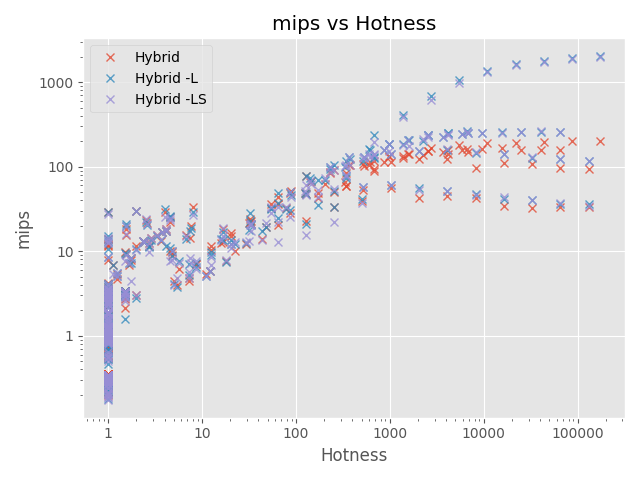
\includegraphics[scale=0.75]{output/graphs/scatter/hybrid/hotness.png}
    \caption{Performance (mips) vs hotness for all tests on the hybrid emulators.}
    \label{figure:hybrid-hotness}
\end{figure}

This is because hybrid behaves like an interpreter for sufficiently cold tests, but like a JIT for sufficiently hot tests. This causes it to exhibit the `flat' performance profile of the interpreter for low hotness, before dropping in performance then rising as the JIT would. The dip in performance or the inflection point is where the hybrid begins to act like a JIT, and thus takes on all the associated overheads of a JIT, without having time make them worthwhile. This region therefore performs worse than both the interpreter or the JIT.

Naturally, we should expect the location of this inflection point to change with \texttt{-T}. Since \texttt{-T} determines how many times a block must be executed before it is compiled, it roughly corresponds to how hot a block should be before the hybrid begins emulating like a JIT; given this, we would expect the inflection to occur at higher hotness values for higher \texttt{-T}.

The ideal value for \texttt{-T} is not something that can be found through intuition; larger values will avoid more unnecessary compilation, but smaller values will cause better utilisation of the worker threads and the JIT compiler's increased execution performance.

One might logically think that the minimum value of \texttt{-T1} would lead to the highest performance on heavy test cases, but this was not found to be the case. \autoref{figure:hybrid-t-primal-mips} shows how the different values of \texttt{-T} perform on the \texttt{primal(n)} test suite.

\begin{figure}[H]
    \centering
    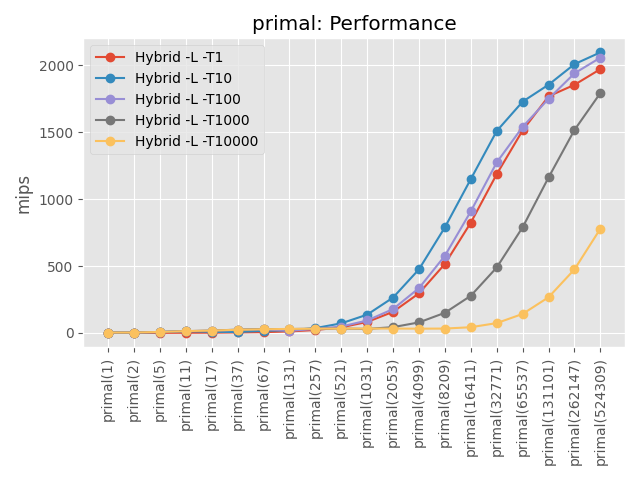
\includegraphics[scale=0.75]{output/graphs/tests/hybrid_t/primal/mips.png}
    \caption{Performance in mips of the primal test suite run on the hybrid emulator with varying values for \texttt{-T}.}
    \label{figure:hybrid-t-primal-mips}
\end{figure}

Interestingly, we observe that \texttt{-T10} has the highest performance for the intensive \texttt{primal(n)} tests; we might expect that \texttt{-T1} would hold this position as that would cause the most aggressive compilation which would eventually lead to the best performance. The most likely explanation is that \texttt{-T1} wastes too much time compiling cold blocks that are executed very infrequently and have no time to pay off (such as the entry point) causing the worker pool to be busy for longer. This would delay the compilation of the hot blocks causing the interpreter fallback to activate more frequently, despite the fact that more blocks are translated overall. We observe that larger values of \texttt{-T} cause steadily worse performance for the more intensive tests, as we might expect.

\autoref{figure:hybrid-t-primal-time} shows the execution times for the same test suite, which helps paint a far clearer picture for the performance characteristics with small \texttt{n}. We observe that \texttt{-T1} is unable to benefit from the low overhead characteristic of the emulator and begins with a relatively high execution time. Furthermore, we can see that the performance at low \texttt{n} is improved as \texttt{-T} is increased. We can see that each curve behaves characteristically like the interpreter, showing a direct proportionality between the performance and \texttt{n} up until an inflection point caused by the hybrid acting more like the JIT emulator. This inflection point is similar to the one observed when investigating the relationship with hotness. Once this point is hit, the execution time becomes fairly constant before eventually curving back into a line just like with the JIT emulator. We can also see that whilst \texttt{-T10} generally performs the best, this is not universal, and it has a sour spot where it has begun compiling more blocks without having any time for it to pay off.

\begin{figure}[H]
    \centering
    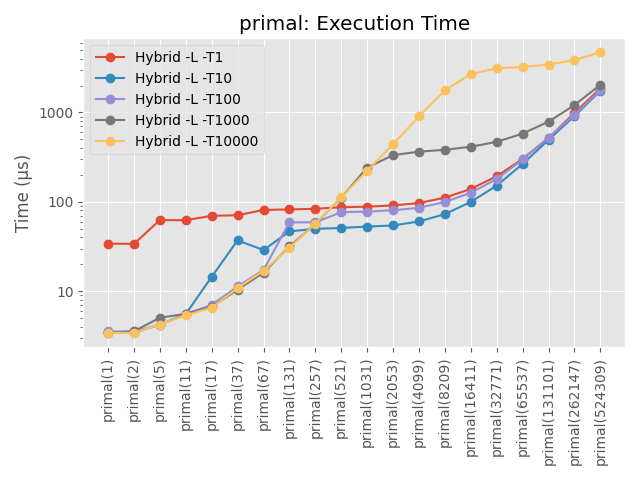
\includegraphics[scale=0.75]{output/graphs/tests/hybrid_t/primal/time.png}
    \caption{Execution time of the primal test suite run on the hybrid emulator with varying values for \texttt{-T}.}
    \label{figure:hybrid-t-primal-time}
\end{figure}

This general effect of \texttt{-T} on the performance characteristics was observed for most other test suites including \texttt{fibonacci(n)} and \texttt{memcpy(n)} as shown in \Cref{figure:hybrid-t-fibonacci-mips,figure:hybrid-t-memcpy-mips}

\begin{figure}[H]
    \centering
    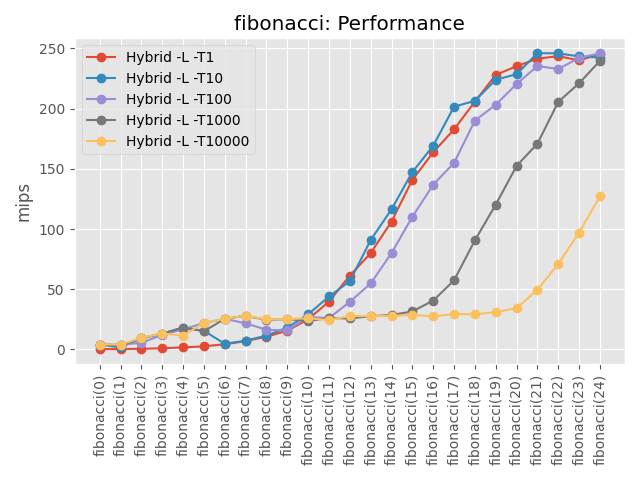
\includegraphics[scale=0.75]{output/graphs/tests/hybrid_t/fibonacci/mips.png}
    \caption{Performance in mips of the fibonacci test suite run on the hybrid emulator with varying values for \texttt{-T}.}
    \label{figure:hybrid-t-fibonacci-mips}
\end{figure}

\begin{figure}[H]
    \centering
    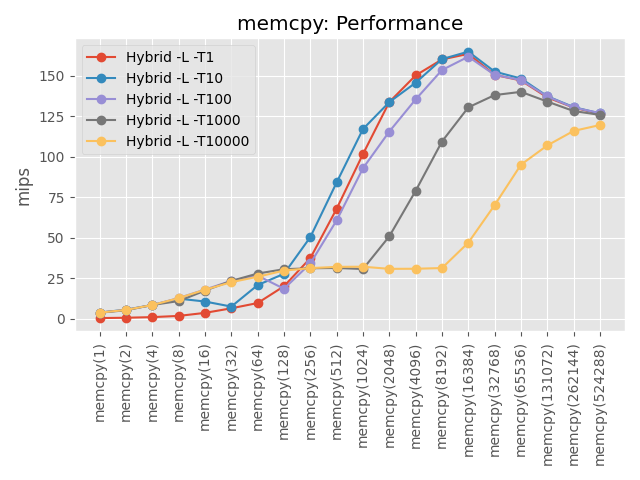
\includegraphics[scale=0.75]{output/graphs/tests/hybrid_t/memcpy/mips.png}
    \caption{Performance in mips of the memcpy test suite run on the hybrid emulator with varying values for \texttt{-T}.}
    \label{figure:hybrid-t-memcpy-mips}
\end{figure}

The optimisation \texttt{-L} was enabled for the hybrid emulator as it produced the same favourable results as with the JIT emulator, as explored in \autoref{section:perf-jit}, for reasons already discussed. The majority of tests saw performance improvements with \texttt{-L} enabled with hotter tests seeing improvements by orders of magnitude whereas shorter tests saw very slight performance degradation.

The next aspect to investigate is the performance characteristics of the hybrid emulator with speculative compilation (\texttt{-S}) enabled. One would expect that it might improve the performance in heavy workloads, as the hybrid will be capable of speculatively compiling blocks before they are first required. 

\begin{figure}[H]
    \centering
    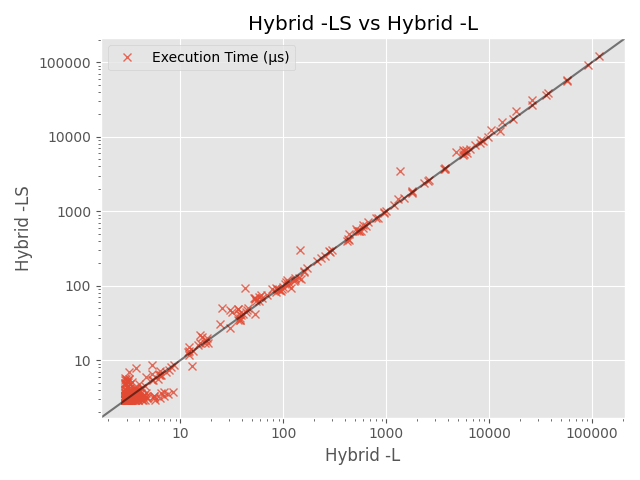
\includegraphics[scale=0.75]{output/graphs/scatter/vs/Hybrid -L-vs-Hybrid -LS-time.png}
    \caption{Execution time of all tests for \texttt{Hybrid -L} vs \texttt{Hybrid -LS}.}
    \label{figure:hybrid-l-vs-hybrid-ls}
\end{figure}

The execution time of all tests run on the hybrid emulator with and without \texttt{-S} is shown in \autoref{figure:hybrid-l-vs-hybrid-ls}; it is unclear from this what difference, if any, \texttt{-S} makes to the performance. In some instances, we see noticeably worse performance with \texttt{-S} enabled, however in the majority of cases there is no significant difference. To obtain a clearer picture, we turn our attention to individual test suites.

\begin{figure}[H]
    \centering
    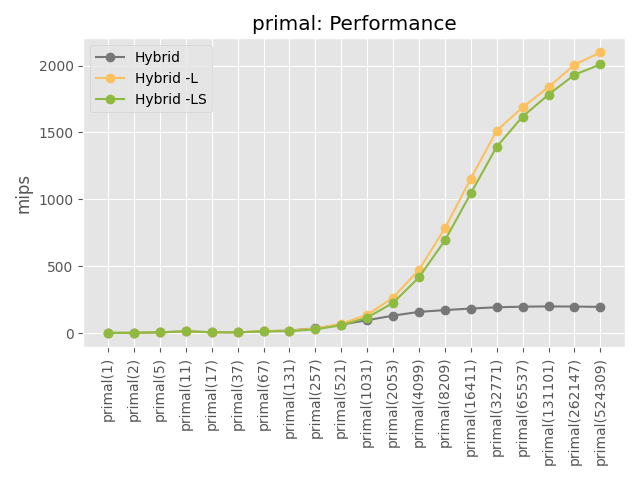
\includegraphics[scale=0.75]{output/graphs/tests/hybrid/primal/mips.png}
    \caption{Performance in mips of the primal test suite run on the hybrid emulator with different optimisations enabled.}
    \label{figure:hybrid-primal-mips}
\end{figure}

\autoref{figure:hybrid-primal-mips} shows the performance of the \texttt{primal(n)} test suite for different configurations of the hybrid emulator. From this, it is clearer that the effect of \texttt{-S} is detrimental; this may seem counterintuitive, but it is likely for the same reason that \texttt{-T10} was better than \texttt{-T1} even for hot workloads, as discussed previously. \texttt{-S} is likely overloading the worker pool with unimportant blocks (even more so, since they may never be executed at all) which delays the compilation of the important hot blocks, despite increasing the total number of compiled blocks.

\begin{figure}[H]
    \centering
    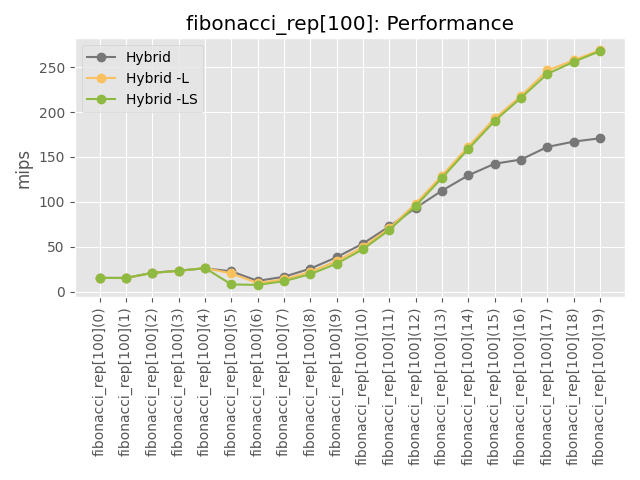
\includegraphics[scale=0.75]{output/graphs/tests/hybrid/fibonacci_rep[100]/mips.png}
    \caption{Performance in mips of the fibonacci\_rep[100] test suite run on the hybrid emulator with different optimisations enabled.}
    \label{figure:hybrid-fibonacci-100-mips}
\end{figure}

In order to determine if \texttt{-S} shows benefit in larger programs we observe the results of the \texttt{fibonacci\_rep[100](n)} test suite shown by \autoref{figure:hybrid-fibonacci-100-mips}. Despite the much larger program size, \texttt{-S} appears to either make no difference or degrade the overall performance. For these reasons, \texttt{-S} should be considered detrimental in its current state and disabled.

With the configuration investigated, we can now move onto comparing the performance of the hybrid emulator with that of the JIT emulator; \autoref{figure:hybrid-l-vs-jit-l-mips} shows the performance of all tests on the hybrid emulator vs the JIT emulator, both with \texttt{-L} enabled.

\begin{figure}[H]
    \centering
    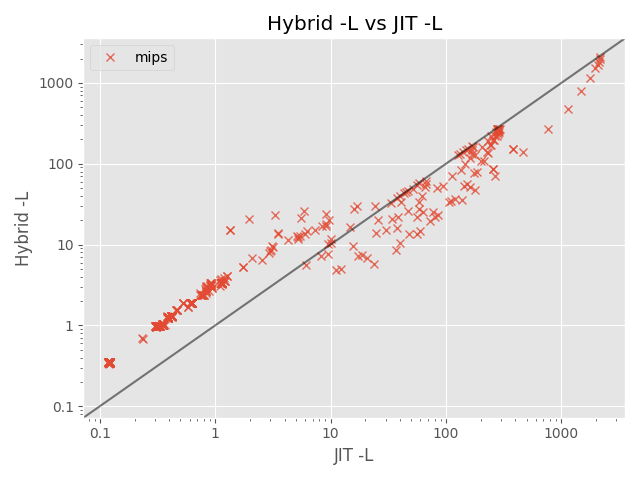
\includegraphics[scale=0.75]{output/graphs/scatter/vs/JIT -L-vs-Hybrid -L-mips.png}
    \caption{Performance in mips of all tests for \texttt{Hybrid -L} vs \texttt{JIT -L}.}
    \label{figure:hybrid-l-vs-jit-l-mips}
\end{figure}

The interesting trend we see in the plot is caused by the same inflection point we observed when comparing the hybrid emulator's performance to program hotness. Programs with lower performance on both the JIT and hybrid emulators tend to have lower program hotness, causing the hybrid to behave more like an interpreter and outperform the JIT emulator. Likewise, programs with higher performance tend to also have higher hotness, and thus the hybrid acts more like a JIT emulator again. This stops the JIT emulator from beating the hybrid by orders of magnitude like it does to the interpreter.

Despite acting like a JIT emulator for hotter tests, we see that the hybrid still performs worse than the JIT emulator (but not nearly as bad as the interpreter); this due to the added overheads and complexities associated with the hybrid emulator. It appears that the utilisation of the worker thread to asynchronously JIT compile blocks whilst executing the program is not able to make up for the increased overheads.

Despite this, the hybrid emulator's performance characteristic is quite desirable compared to the interpreter; when it loses to the JIT emulator it is never by more than an order of magnitude, unlike the interpreter. While the hybrid sacrifices peak performance over the JIT emulator at the high end, it arguably makes up for it by considerably improving the performance at the low end, resulting in more consistent performance across the board.

\begin{figure}[H]
    \centering
    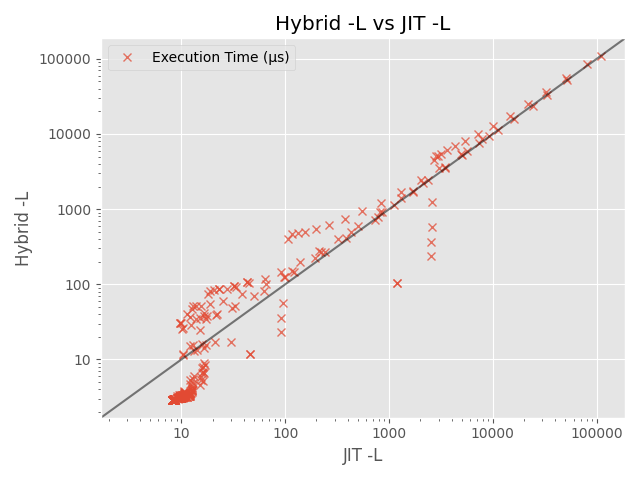
\includegraphics[scale=0.75]{output/graphs/scatter/vs/JIT -L-vs-Hybrid -L-time.png}
    \caption{Execution time of all tests for \texttt{Hybrid -L} vs \texttt{JIT -L}.}
    \label{figure:hybrid-l-vs-jit-l-time}
\end{figure}

\autoref{figure:hybrid-l-vs-jit-l-time} shows the execution time of all tests for both the hybrid and JIT emulators and shows a similar picture. Shorter tests tend to run faster on the hybrid emulator, especially at the low end, whereas longer tests tend to perform better on the JIT emulator; in the majority of cases the performance of both emulators is on the same order of magnitude.

The ideal configuration found for the hybrid emulator is detailed in \autoref{tbl:hybrid-optimal}

\begin{table}[H] 
    \centering
    \begin{tabular}{l|c}
        \toprule
        Option & Value \\
        \midrule
        \texttt{-L} & \cmark \\
        \texttt{-S} & \xmark \\
        \texttt{-T} & 10 \\
        \bottomrule
    \end{tabular}
    \caption{Optimal configuration found for the hybrid emulator.}
    \label{tbl:hybrid-optimal}
\end{table}